% Chapter 3

\chapter{Concept} % Write in your own chapter title
\label{Chapter3}
\lhead{Chapter 3. \emph{Concept}} % Write in your own chapter title to set the page header

Conceptually, SPolly is divided into a speculative loop parallelizer 
and a non-speculative extension to Polly. Even if the objectives for both parts 
are the same, namely to improve the performance of loops, the approaches to accomplish 
them are different. While the former one will introduce speculative parallelism
for promising loops at runtime, the latter one tries to weaken the harsh 
requirements on SCoPs in order to make Pollys loop optimizations applicable on
a wider range of loop nests. In the presented setting both approaches may benefit
from the polyhedral optimizations and also from parallel execution, so it is 
hardly surprising that the polyhedral analyses play a decisive role. 
On the one hand they reveal loop nests which may be optimized by Polly, with or
without the extensions of SPolly, on the other hand they are used to detect 
promising loops to speculate on.
Apart from the implementation work, which will be described in the 
next Chapter, this thesis presents the concepts and key ideas to accomplish both
stated goals.
We believe that these ideas and the gained knowledge is very 
valuable not only for future work on SPolly  but also for
other approaches facing similar situations.

%On the way to a working version 
%many pitfalls have been encountered that should be avoided in the future, 
%perhaps with similar approaches we worked out. 




\section{Speculation in the Polytope Model}
One great benefit of Polly and the underlying polyhedral model
is to detect and model loop carried data dependencies. Regarding this fact it
sounds plausible to use this ability in a speculative context as well.
Unfortunately speculative 
extensions will compromise this ability because they will assume
less dependencies when they weaken the requirements. As less dependencies may
lead to more transformations, any speculative extension has to keep track of 
 any change, e.g., to the iteration space, in order to preserve the semantics 
once the speculation fails. It is beyond the scope of this work to allow 
arbitrary polyhedral transformations with speculatively removed dependencies, 
so a more conservative way was chosen and implemented. 
At first, non-computable memory accesses, as they may arise from  
aliases or function calls, are overestimated. 
The resulting polyhedral model is complete with regard to possible
data dependencies, but could still reveal e.g., a scheduling for 
better data-locality or possible vectorization. 
Afterwards speculation is applied or in other words, the optimized loop nest is
speculatively  parallelized. 
Note here, that Polly can only change the scheduling based on the
overestimated and therefore complete polyhedral representation of the loop nest,
thus only in a sound way. A more detailed description on both steps is given
in the following Sections, especially \ref{SpeculativeParallelExecution},
\ref{SpeculationFreeOptimizations} and \ref{OverestimatingDependencies}.

\section{Speculative Static Control Parts}
\label{sSCoPs}
As Polly is restricted to static control parts, there is a counterpart limiting
the applicability of SPolly. This counterpart is called 
speculative static control part, or short sSCoP. Both are the central entities of 
the respective tool and they only differ in the restrictions on the underlying region.
In contrast to Polly, SPolly allows arbitrary function calls, possible aliases
and non-affine base pointers of memory accesses.   

To illustrate the differences, Figure \ref{fig:WeakendSCoPs} presents three 
sSCoPs where each one validates one of the weakened restrictions,
thus is a sSCoP but no SCoP. As a comparison
to the restrictions on SCoPs (Table \ref{tab:SCoPRestrictions}), a full list
of sSCoP restrictions is given in Table \ref{tab:sSCoPRestrictions} on page 
\pageref{sSCoPRestrictionsPage}.

\lstset{frame=none}
\begin{figure}[htbp]
  %\begin{framed}
  \vspace*{-5mm}
  \centering
  \subfloat[Speculative static control part violating the function call restriction on SCoPs]{
    \begin{minipage}[c][3.5cm]{0.3\textwidth}
      \begin{tabular}{c}
      \lstinputlisting{Primitives/Code/sSCoP1.c}
      \end{tabular}
      \label{lst:sSCoP1}  
    \end{minipage}
  }
  \subfloat[Speculative static control part violating the aliasing restriction on SCoPs]{
    \begin{minipage}[c][3.5cm]{0.33\textwidth}
      \begin{tabular}{c}
      \lstinputlisting{Primitives/Code/sSCoP2.c}
      \end{tabular}
      \label{lst:sSCoP2}  
    \end{minipage}
  }
  \subfloat[Speculative static control part violating the base pointer restriction on SCoPs]{
    \begin{minipage}[c][3.5cm]{0.3\textwidth}
      \begin{tabular}{c}
      \lstinputlisting{Primitives/Code/sSCoP3.c}
      \end{tabular}
      \label{lst:sSCoP3}  
    \end{minipage}
  }

  \caption[Speculative valid static control parts (sSCoPs)]{Speculative valid static control parts (sSCoPs), each violating one restriction of static control parts (see Section \ref{SCoPs}, especially Table \ref{tab:SCoPRestrictions})}
  \label{fig:WeakendSCoPs}
  %\end{framed}
\end{figure}
\resetlst

\section{Speculative Parallel Execution}
\label{SpeculativeParallelExecution}
Speculative loop parallelization is one of the two major purposes of 
SPolly. The challenge is to exploit as much parallelism as possible 
without restricting the applicability too much. In the context of this work, 
we limit ourselves to speculative valid SCoPs as described in the last Section. 
This restriction allows us to derive certain assumptions similar to the ones 
Polly requires. As a result, we are able to utilize main parts of Polly including 
the polyhedral representation. It is used to detect speculatively parallelizable loops 
without risking too much misspeculations. 
Before a sSCoP is parallelized the loop carried dependencies for each loop 
are computed as they would be in a non-speculative context.
The used polyhedral model differs from the one
created for an ordinary SCoP because it does not represent all possible memory accesses,
thus it is incomplete.
Even if aliasing pointers may access the same memory address, SPolly 
speculatively ``removes'' the dependencies between possibly aliasing base pointers
when the polyhedral representation is created. Furthermore, all possible effects
of a function call are ignored in this step. This includes
memory effects as well as observable behaviour.
Those differences prevent us from using the ``normal'' polyhedral transformations 
in order to increase data-locality, because they could alter the iteration order.
Even if we use an extended STM to guard the execution, it is crucial to preserve
the initial order for sound speculative parallelization. If not,
a commit order could not prevent that the STM allows the wrong 
transaction to commit its results once a conflict is detected. Otherwise, if
the initial order is maintained, hence all memory effects applied as in a sequential 
execution, only the observable behaviour of function calls 
can cause unsound results. To prevent this, the described wait construct 
is introduced right before the first call instruction on each execution path, 
thus functions will be executed only after all former changes have been 
synchronized. Because those wait constructs will create
mutual exclusive (or non-parallel) sections, this speculative approach promises 
better results when the function calls are executed less frequently, e.g., like
error handling code. 

An example illustrating the need of a commit order and the preservation of the 
initial order is given in Section \ref{NonComputableDependenciesExample}.


\subsection{Sequential Consistency}
As speculative execution implies the possibility of misspeculation, actions have
been taken to preserve the semantic of each speculatively parallelized loop nest.
As explained in the last Chapter, Sambamba uses an STM as conflict management system 
for speculative execution. In the current (not extended) implementation, the STM 
is not able to resolve conflicts between iterations executed in parallel in a 
proper way. If two transaction interfere the STM might allow the later one
(in terms of the original iteration order) to commit its result before the 
former one could. As this one will be forced to roll back and recompute, 
it has to use the corrupted, but permanently written,
data resulting from the committed computation. Because this does not preserve the 
semantics in each case, it is important to prevent such cases from happening. For
most of the introduced speculations a commit order will suffice, but arbitrary 
function calls need the described wait construct too. It is also crucial that
the initial order is only changed in the non-speculative setting, because otherwise
the commit order would become futile and the described problem arises again.
Later on (Section \ref{SpeculationFreeOptimizations}) we will describe how
polyhedral transformations on sSCoPs can be applied in a sound way, 
even if they change the iteration order. 

Assuming that all transactions are committed in a ``proper order'' and function 
calls are guarded by wait constructs,
we state that the speculatively parallelized loop will always yields a
sound result. To support this statement the following three paragraphs will
present argumentations which successively back up the soundness of the described 
speculations. The first one also defines the ``proper order'' we assumed. 

\paragraph{Aliasing pointers} ~\\
Given a valid SCoP, but with possibly aliasing pointers 
(for example Figure \ref{lst:sSCoP2}), 
SPolly may speculatively parallelize the loop and therefore execute iterations in 
parallel which access the same memory addresses. 
As the STM will by construction detect all memory access conflicts,
it will also detect those emerging from aliases.
We assume that such conflicts will be resolved based on a commit order which
correlates with the iteration order of the parallelized loop. 
This is ensured, because the commit order 
(once it is available) is filled by unrolled iterations 
in their initial order (see Section \ref{CodeGeneration} for details).
We can conclude that in the case of a memory conflict, 
the transaction prior in the loop order is allowed to commit its
changes, whereas the other conflicting (and later) ones are forced to roll back.
Thus, the first transaction (corresponding to the first iteration)
can always commit its results and the later ones 
will respect the iteration order of the loop in the case of a conflict. 
Inductively, the soundness of the speculative parallelization can be concluded
if the iteration order of the loop nest was only transformed in a non-speculative 
context (e.g., not transformed at all). 


\paragraph{Non-affine base pointers} ~\\
Non-affine base pointers include loop dependent ones (as in Figure \ref{lst:sSCoP3}),
but also those returned by functions or computed in another non-affine way. 
In any case the soundness argument follows from the one given for 
aliasing instructions. Non-affine base pointers can be seen as start address of
an unknown array. This array may alias with every other memory address, thus
all accesses to this array may alias with all other memory accesses within the 
sSCoP. At this point the line of argument presented in the last paragraph 
fits again. 

\paragraph{Arbitrary function calls} ~\\
Speculative execution of arbitrary function calls causes three main problems you
have to cope with. First there are memory accesses, but in our case the
argumentation of the last two paragraphs holds here too. 
Apart from that, non-termination and other observable behaviour is possible.
At the moment, we do not (seriously) analyze the called functions, thus we have to
assume each of them may not terminate or cause  observable effects.
With this assumption speculative execution becomes impossible, 
we might want to allow such function calls. As speculative execution is not an
option we have to stop it right before a call and ensure the whole program is in a
state it would be in when executed non-speculative. To do so, the wait construct
described in the context of the STM can be used. Placed right in front of the 
first call instruction on each path,
the executing thread is only allowed to pass if  all prior iterations
(in terms of the non-speculatively changed iteration order) have been completed and the
current state of the waiting thread is not conflicting with any of the previous 
commits. The wait construct will pause the thread until the first condition is
fulfilled and then check if the second one holds too. If so, the thread might pass,
otherwise the current transaction will be rolled back, but with the guarantee that 
this time no STM synchronization problem can occur. 


\subsection{Possible Misspeculations}
Misspeculations as such occur when speculatively removed dependencies emerge during
the execution. In the context of this work, also executed call instructions could
be considered misspeculations. In both cases the current computation might be
discarded, however,  this is not always necessary. Even existing dependencies could
allow speculative execution as long as the memory accesses follow the earlier 
stated ``proper order''.
But since this depends only on the scheduling of the threads, we have to assume all 
misspeculations as fatal.
The worst case would force each succeeding iteration, speculatively 
executed in parallel, to roll back and recompute,
once another one committed its results. 
The processor time overhead would be quadratic in the number 
of parallel executed transactions. This includes the memory access logging,
the synchronization and the performed rollbacks.
As countermeasure, SPolly monitors the runtime of all speculatively parallelized
sSCoPs and reverts the speculation for poorly performing ones. Future work could
minimize the overhead of monitoring by 
instrumenting the parallelized sSCoP (or the STM) in order to notify SPolly 
if the number of rollbacks exceed a certain threshold. 

%In a worst case scenario the execution time raises by a factor quadratic in the
%number of parallel executed transactions plus the overhead introduced by the STM. 

%\subsection{Advantages}
%In contrast to the speculation free optimization approach, this one is also
%capable of parallelizing sSCoPs with almost arbitrary function calls. To do so the
%STM has to provide the  wait construct as described earlier. 
%Even if this is not yet the case, SPolly could introducing such wait with no 
%further effort. 
%This will certainly cause additional overhead during the parallel execution, 
%but it does not preclude a performance gain per se.

%In the special case of sSCoPs, we know certain things about the 
%control flow and the memory accesses within a parallelized region. 
%With the assumptions we may derive from the requirements on sSCoPs it is possible
%to secure the speculative parallel execution by introducing wait constructs 
%right before each possibly violating function call. Executing those function calls
%in the correct order will enforce all their possible effects to be applied 
%in the correct order too. 
%If arbitrary control flow and conditionals are allowed, this conclusion does not
%hold anymore. In fact every memory access could change the taken execution path of 
%another thread, thus every branch would need special annotations. 



\section{Speculation Free Optimizations}
\label{SpeculationFreesSCoPs}
\label{SpeculationFreeOptimizations}
As second objective, SPolly may enable sound polyhedral optimizations, even
parallelization, on sSCoPs. Because there is no need for speculation at all, this
kind of optimization could be applied even without the presence of Sambamba and 
the included STM.
In the following we will introduce tests initially designed to lower the rate 
of misspeculations but sometimes powerful enough to completely rule out violations
on sSCoPs. In such cases SPolly can use the code generation of Polly to 
exploit parallelism and the tests to preserve the semantics. Apart from these cases,
it is possible to overestimate possible data dependencies in order to obtain a
complete and sound polyhedral representation. Section \ref{OverestimatingDependencies}
describes the latter approach while the next Section will cover the introduced checks.

%Further details on both cases are
%given in the sections \ref{IntroducedTests} and \ref{OverestimatingDependencies},
%respectively.





\section{Region Scores}
\label{RegionScores}
\lstset{frame=none}
\begin{figure}[h]
  %{r}{0.4\textwidth}
  \centering
  \subfloat[Complete static sSCoP]{
    \begin{minipage}[c][2cm]{0.45\textwidth}
      \lstinputlisting{Primitives/Code/sSCoPstatic.c}
      \label{lst:sSCoPstatic}  
    \end{minipage}
  }
  \subfloat[sSCoP with variable loop bounds and a function call]{
    \begin{minipage}[c][2cm]{0.45\textwidth}
      \lstinputlisting{Primitives/Code/sSCoPbounds.c}
      \label{lst:sSCoPcall}  
    \end{minipage}
  }

  \subfloat[Branch within a sSCoP]{
    \begin{minipage}[c][3cm]{0.45\textwidth}
      \lstinputlisting{Primitives/Code/sSCoPbranch.c}
      \label{lst:sSCoPbranch}  
    \end{minipage}
  }
  \subfloat[Observable call within a sSCoP]{
    \begin{minipage}[c][3cm]{0.45\textwidth}
      \lstinputlisting{Primitives/Code/sSCoPprintf.c}
      \label{lst:sSCoPprintf}  
    \end{minipage}
  }
  \caption{Examples for speculative valid static control parts (sSCoPs)}
  \label{fig:ScoredSCoPs}
\end{figure}
\resetlst
Region scores are used as a heuristic to decide whether or not an sSCoP is worth
to speculate on, thus for which regions profiling and optimized versions should
be created and as a result executed.
As profiling may change the score again it is reasonable to create 
optimized versions only if the profiling results suggest to do so. 
It is obvious that we want to consider only loops and loop nests of a certain size,
thus profiling the trip count may have enormous impact on the actual region score.
Additionally we are interested in execution paths within an sSCoP in order
to predict how often
e.g., irreversible instructions, may be executed. While such instructions, like
calls to \texttt{printf}, may cause STM rollbacks during the parallel executions
(after the wait construct failed synchronizing with previous commits),
branch probabilities may also have a huge impact on the actual sSCoP size and
only rarely occurring dependencies. 

To clarify the idea, the regions scores for the Figure \ref{lst:sSCoPstatic}
to \ref{lst:sSCoPprintf} are given in Table \ref{tab:Scores}. 
Some of the constants in the presented scores are fixed, e.g., to 
weight trip counts, but others are dynamically 
computed from the given sSCoP size and the contained instructions. The variables
can also be divided into those representing sSCoP invariant parameters 
(\texttt{N} and \texttt{M}) and symbolic values to take 
e.g., branch probabilities into account. 
Later on, both kinds will be instantiated with profiling data, e.g., the 
execution probability of a branches consequence or alternative,
which results in an actual integer score. 

%\paragraph*{Example} ~\\
Considering Figure \ref{lst:sSCoPbranch}. Starting leftmost we can
see the weighted loop trip count of 64 which is the quotient of the actual trip
count 1024 and the constant 16. This ensures that loops with less then 16 iterations will not 
be scored positive.
The outermost expression enclosed in parenthesis 
is the region score of the whole loop body. First, the 11 instructions of the always 
executed branch condition and afterwards the branch structure is taken into account.
Two symbolic variables, namely  ``@if.then\_ex\_prob'' and ``@if.else\_ex\_prob'',
have been inserted and they will be instantiated with the 
profiled execution probabilities for the conditional. The instantiation for all 
symbolic variables will be done by the runtime part of the SPolly module,
first with sample values, e.g., fifty percent execution probability for each branch,
and later on with the real profiled execution probabilities and loop trip counts. 
Within the two branch subexpressions the numbers 5 and 7 
denote the size and the 100 weights
the execution probability which was given in per cent. For this example all
instructions are of the same weight, hence the region score will yield the number
of executed instructions once two probabilities are given. 
In fact it will only be one-sixteenth as the loop trip counts have been weighted. \\

\begin{table}[htbp]
  \begin{framed}
  \centering
  \caption{Region scores for the sSCoPs presented in Figure \ref{fig:ScoredSCoPs}}
  \begin{tabular}{ c c}
    Figure & symbolic region score \\
    \hline
    %\ref{lst:ExampleLoopNest} & $ 408 $ \\
    \ref{lst:sSCoPstatic} & $ 576 $ \\
    %\hfill \text{  (if \texttt{A,B} and \texttt{C} may alias)} $ \\
    \ref{lst:sSCoPcall} & $\%\texttt{N} / 16 * (7 + (10 * (\%\texttt{M} / 16)))$ \\ 
    \ref{lst:sSCoPbranch} & $64 * (11 + (7 * \text{@if.then\_ex\_prob} / 100) + (5 * \text{@if.else\_ex\_prob} / 100)) $ \\
    \ref{lst:sSCoPprintf} & $\%\texttt{N} / 16 * ((6 * \text{@if.else\_ex\_prob} / 100)  + (-100 * \text{@if.then\_ex\_prob} / 100))$ \\
    %\ref{lst:AliastestAccessesSrc} & $  (7 + ((8 + (8 * (\%\text{N} / 16))) * (\%\text{N} / 16))) * ((0\text{ smax \%N}) / 16) $ \\

   \end{tabular}
  \label{tab:Scores}
\end{framed}
\end{table}


%\clearpage

\section{Introduced Tests}
\label{IntroducedTests}
The already mentioned tests were initially designed as an attempt 
to keep the rate of misspeculations low. As such, they are used to 
refine region scores in the context of profiling, 
but it turned out that they can be of great use in optimized versions too.
At the moment SPolly is capable of creating two different kinds of checks.
If they rule out SCoP violations completely we may call them complete. 
For such cases the optimized versions with the introduced checks will always 
yield a  sound result, hence there is no need for speculation at all. 
%As such cases can improve the applicability of Polly even without an STM, 
%they could find their way into the main branch one day.

To place the tests we take advantage of Pollys default behaviour which is to 
copy the optimized SCoP as an alternative to the
original one. Figure \ref{fig:PollySCoPCFG} shows the CFG after Polly optimized
a given SCoP. The dotted edge is not taken since the guard of the conditional in
the split block is constant true. 
In the SPolly version this guard is replaced by the actual test result as 
indicated in Figure \ref{fig:SPollySCoPCFG}.

\begin{figure}[htbp]
  \centering
  \subfloat[CFG after optimization with Polly]{
    \begin{minipage}[c][1\width]{0.5\textwidth}
    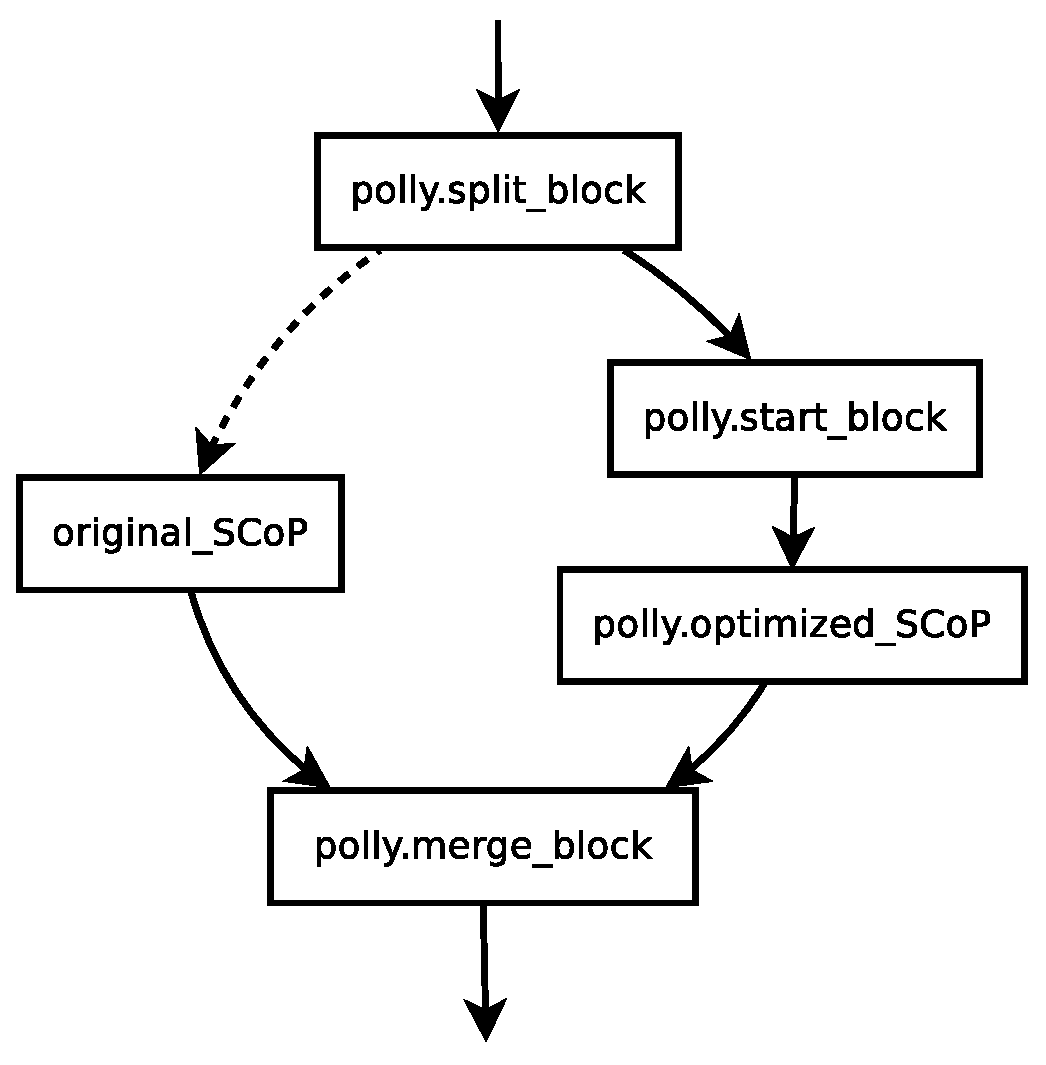
\includegraphics[width=0.9\textwidth]{Figures/PollySCoPCFG.eps}
    \label{fig:PollySCoPCFG}
    \end{minipage}
  }
  \subfloat[CFG after optimization with SPolly]{
    \begin{minipage}[c][1\width]{0.5\textwidth}
    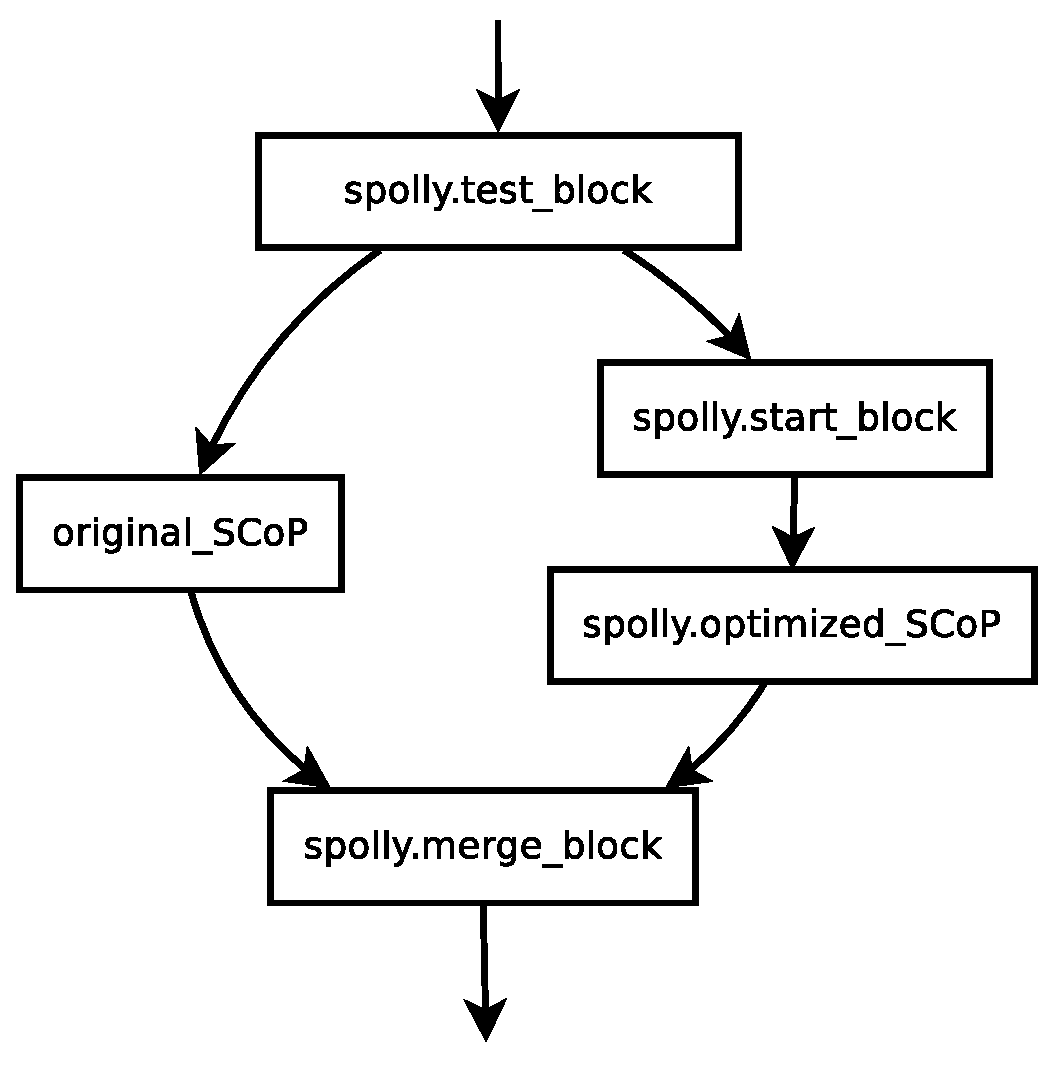
\includegraphics[width=0.9\textwidth]{Figures/SPollySCoPCFG.eps}
    \label{fig:SPollySCoPCFG}
    \end{minipage}
  }
  \caption{CFG produced by Polly and SPolly, respectively}
  \label{fig:SCoPCFG}  
\end{figure}





\subsection{Alias Tests}
Testing for aliasing pointers in general would be quite expensive because 
there could be aliasing between every possible pair. As this includes
also the loop dependent pointers we would need to compute them beforehand in order 
to compare them pairwise. With this in mind, we decided to test only sSCoP
invariant pointers, once before the sSCoP is entered. 
If the test succeeds, thus no aliases are found, the optimized version
is executed, otherwise, the unoptimized sequential one. 
At compile time the accesses for each base pointer are collected and
marked either as possibly minimal, possibly maximal or not interesting access. 
Accesses are called possibly maximal (minimal) if there is no other access to this base 
pointer which is statically known to be greater (less) in terms of integer arithmetic. 
At runtime all possibly minimal and maximal accesses are respectively compared until,
in the end, the minimal and the maximal access for each base pointer is computed.
The alias test as such compares again the minimal access for a base pointer with the maximal 
accesses for each other base pointer and vice versa. After this comparison chain the 
result may indicate or rule out aliasing between them. 
If all base pointers are invariant in the SCoP the test is complete,
thus aliasing can be ruled out for the sSCoP at runtime. 

%However, non-invariant pointers are not tested at all, as it would 
%imply to perform all computation and testing within the loop. 

%Figure \ref{fig:AliastestConcept} illustrates the concept of the alias
%tests while listing \ref{lst:AliastestAccessesSrc} and table
%\ref{fig:AliastestAccesses} provide an example loop nest and the corresponding 
%minimal and maximal memory accesses. 
%The alias test for this example would look similar to the one presented in listing
%\ref{lst:AliastestAccessesOut}. 
%Figures \ref{fig:AliastestOverview} and \ref{fig:Aliastest} provide an overview 
%of the aliastests and example, respectively. 
%To get a better understanding we will now discuss them in more detail.

%\paragraph*{Example} ~\\
Figure \ref{fig:AliastestConcept} shows three arrays with their base pointers 
(bp) and the minimal (maximal) access, denoted by ma and Ma, respectively. 
Two of the six comparisons needed to rule out aliasing for these arrays  
are indicated by arrows. The other four also compare a minimal
and maximal accesses for different base pointers. 
As shown, the minimal accesses might be at the base pointer but also in front of it.
This is the case if the base pointer is e.g., not the beginning of an array.

Part {\footnotesize{A}} of Figure \ref{fig:Aliastest} 
shows the matrix multiplication example which will be discussed
further in Chapter \ref{Chapter6}. Assuming that the arrays are statically 
flattened, the loop nest contains four accesses. Such flattening is done by the 
compiler if the array is multidimensional but of a statically known size
(see Section \ref{CaseStudyCaseA}). Within Polly 
the accesses are analyzed and matched to their base pointers, here \texttt{A},
\texttt{B} and \texttt{C}.  SPolly will statically analyse them too, in order to
find all possible minimal and maximal accesses. In this case both types can be
statically reduced to a unique offset as shown in part {\footnotesize{B}}. 
Acc denotes the access as named in the source code,
bp the base pointer, ma the minimal access and Ma the 
maximal one. Comparing them will rule out aliasing for the loop nest
completely because no base pointer is loop dependent. The last part
({\footnotesize{C}}) shows the actual alias test (or the comparison chain)
SPolly introduces and the result which is used
to choose whether or not to execute the speculatively optimized version.



\lstset{frame=none}
\begin{figure}[htbp]
  \centering
  %\subfloat[Alias test from a birds eye view]{
  %\begin{minipage}[c][4cm]{\textwidth}
    \includegraphics[width=0.9\textwidth]{Primitives/aliastest.eps}
  %\end{minipage}
  \caption{Alias test from a birds eye view}
  \label{fig:AliastestConcept}  
  %}
\end{figure}

\begin{figure}[htbp]
  \centering
  %\vspace*{2mm}
  \subfloat[sSCoP with possibly aliasing accesses (I1 to I4)]{
    \begin{minipage}[c][4cm]{0.5\textwidth}
    \lstinputlisting{Primitives/Code/aliastestbsp.c}
    \end{minipage}
    \label{lst:AliastestAccessesSrc}  
  }
  \subfloat[Statically derived min/maximal accesses]{
    \begin{minipage}[c][4cm]{0.4\textwidth}
    \vspace*{-2mm}
    \centering
    \begin{tabular}{ c c c c }
      Acc & bp & ma & Ma \\
      \hline
      I1 and I2 & C & 0 & N$ * $N$ - 1$ \\ 
      %I2 & C & 0 & N$ * $N$ - 1$\\ 
      I3 & A & 0 & N$ * $N$ - 1$\\ 
      I4 & B & 0 & N$ * $N$ - 1$\\ 
    \end{tabular}
    \end{minipage}
    \label{fig:AliastestAccesses}  
  }
  
  \subfloat[Introduced alias test compare chain]{
    \begin{tabular}{c}
      \lstinputlisting{Primitives/Code/aliastestout.c}
    \end{tabular}
    \label{lst:AliastestAccessesOut}  
  }
  \caption{Alias tests concept and example}
  \label{fig:Aliastest}  
\end{figure}
\resetlst





\subsection{Invariance Tests}
Apart from alias tests, SPolly may introduce invariance tests if there are
possibly invariant variables and function calls within an sSCoP. The key idea is 
is to monitor possible changes to the variables during the execution of the 
sSCoP. Even if these checks are not complete, they may give hints on dependencies 
between iterations. 
During the execution of the profiling version the test results are gathered 
and then used to influence the region score as the alias test results do.
Initially designed as an exclusion criterion, the invariance tests also provide
useful information about the variables. Such information could be used to
create specialized sSCoP versions in the future.

Figure \ref{lst:InvariantTestSRC} gives an example of an sSCoP 
for which invariance tests can be introduced and \ref{lst:InvariantTestOut} shows
the modified source. Note here that changes to the variable \texttt{c}
during the last iteration are not
monitored. 

\lstset{frame=none}
\begin{figure}[htbp]
  \centering
  \subfloat[Loop nest with possibly invariant variables]{
    \begin{minipage}[c][0.55\width]{0.45\textwidth}
    \lstinputlisting{Primitives/Code/InvariantTestSRC.c}
    \label{lst:InvariantTestSRC}
    \end{minipage}
  }
  \hspace*{5mm}
  \subfloat[Loop nest with invariance tests]{
    \begin{minipage}[c][0.55\width]{0.45\textwidth}
    \lstinputlisting{Primitives/Code/InvariantTest.c}
    \label{lst:InvariantTestOut}
    \end{minipage}
  }
  \caption{Invariance test introduced by SPolly}
  \label{lst:InvariantTest}  
\end{figure}
\resetlst






%\section{Irreversible Function Calls}
%Parallelizing loops containing function calls is a challenge on its own. 
%The called functions may have not computable side effects or they might just 
%print something on your screen. In both cases the order is important and 
%parallel execution becomes unlikely especially if these calls are placed on all
%execution paths. On the contrary there are loops which will execute such
%calls only rarely e.g., as part of error handling. SPolly locates all calls and
%allows loops which execute them only under certain conditions.
%[TODO gefaellt mir nich]






\section{Non-Computable Dependencies}
\label{NonComputableDependencies}
Ruling out may-aliases due to checks was already described earlier, 
but the approach is not feasible in every situation. 
Assuming the example in Figure \ref{lst:NonComputableDependenciesSrc}
we may check if \texttt{A} and \texttt{B} alias in front of the loop nest, but
every array \texttt{A[i]} and \texttt{B[i]} may also alias. 
Introducing tests within the loop nest would not only cause additional overhead 
every iteration but also prohibit the speculative optimization and parallelization
of the outer loop. 
%As in the presented example type
%based alias analysis information could lift the computation of \texttt{A[i]} and \texttt{B[i]} 
%to the outer loop, the innermost one would become a valid SCoP after checks are
%introduced.
At the moment, SPolly is not capable of detection and deciding if 
such a proceeding could be profitable, but instead it tries to optimize and 
speculate on the whole loop nest or to be more precise, on the maximal valid sSCoP.
As mentioned earlier, overestimating such data dependencies could allow
sound polyhedral transformations before SPolly will speculatively execute the
loop nest in parallel. While further details on the overestimation are given in 
the next Section, we will now look at the example in more detail and explain why 
even an STM based approach can produce wrong results when no commit order is available.
\label{NonComputableDependenciesExample}
Assuming we would translate the loop to the pseudo parallelized version in Figure 
\ref{lst:NonComputableDependenciesBad} with the corresponding ParCFG as illustrated 
by Figure \ref{fig:NonComputableDependenciesParCFG}. An input such as the one 
in Figure \ref{fig:NonComputableDependenciesSituation} could now produce wrong 
results even if an STM is used. In the speculatively parallelized versions two
transactions (threads) would work on the same int array because \texttt{A[0]} and 
\texttt{A[1]} are equal. As both transactions read and write the same locations
(\texttt{A[0][0]} to \texttt{A[0][1023]}), the STM will detect
a conflict when the second transaction commits its results. As transaction 1 
(see comment in Figure \ref{lst:NonComputableDependenciesBad}) might commit 
after transaction 2 when no commit order is present, the STM will force a rollback
of transaction 1 once the memory conflict is detected. Unfortunately, this will 
not yield a proper result as the second transaction already altered the state 
of \texttt{A[0] = A[1]} permanently. Introducing a commit order will always 
ensure the original iteration order for STM commits. In this example only 
transaction 2 could be forced to rollback and the overall result would always be 
valid.


\lstset{frame=none}
\begin{figure}[htbp]
  \centering
  \subfloat[Loop nest with non-computable dependencies]{
    \begin{minipage}[c][45mm]{0.45\textwidth}
    \lstinputlisting{Primitives/Code/NonComputableDependencies.c}
    \end{minipage}
    \label{lst:NonComputableDependenciesSrc}  
  }
  \subfloat[Possible input situation for Figure \ref{lst:NonComputableDependenciesBad}]{
    \begin{minipage}[c][45mm]{0.5\textwidth}
    \hfill\hfill
    \includegraphics[width=0.8\textwidth]{NonComputableDependenciesSituation.eps}
    \hfill\hfill
  \end{minipage}
  \label{fig:NonComputableDependenciesSituation}  
  }
  
  \subfloat[Loop nest \ref{lst:NonComputableDependenciesSrc} pseudo parallelized]{
    \begin{minipage}[c][80mm]{0.45\textwidth}
    \lstinputlisting{Primitives/Code/NonComputableDependenciesBad.c}
    \end{minipage}
    \label{lst:NonComputableDependenciesBad}  
  }
  \subfloat[ParCFG for Figure \ref{lst:NonComputableDependenciesBad}]{
    \begin{minipage}[c][80mm]{0.5\textwidth}
    \hfill\hfill
    \includegraphics[width=0.8\textwidth]{NonComputableDependenciesParCFG.eps}
    \hfill\hfill
  \end{minipage}
  \label{fig:NonComputableDependenciesParCFG}  
  }

  \label{fig:NonComputableDependencies} 
  \caption{Example for non-computable dependencies and a violating input}
\end{figure}
\resetlst


%\clearpage


\subsection{Overestimating Dependencies}
\label{OverestimatingDependencies}
Enabling polyhedral optimizations for a wider range of programs is possible, even
if no precise data dependency information can be computed statically. In the case
of non-affine memory accesses Polly assumes all possible addresses, 
reachable from the base pointer, to be accessed. For non-computable dependencies
arising from possible aliases (which includes loop dependent base pointers)
SPolly uses a similar, conservative approach. When the polyhedral description is
computed, dependencies between all possible aliasing base pointers are added. 
Even if this restricts transformations, there is the chance to allow some. 
Loop nests could be for example tiled, despite the fact that there are aliases 
between used base pointers. It is worth to empathize that 
these transformations are completely speculation free because they 
are based on an overestimated, hence complete, polyhedral model.




\section{Method Versioning}
Method versioning is a key feature of the Sambamba framework, but 
not fully implement yet. However, SPolly is already capable of generating a 
profiling and an optimized sSCoP version. As Sambamba will take care of
profiling and dispatching versions in the near future, SPolly can be extended
to create multiple other sSCoP versions without much effort. In this context
profiling data will become even more valuable. Specialized sSCoP versions e.g.,
where we assume constant instead of variable loop bounds,  are one possible usage. 
This would not only 
speed up the execution, but also improve transformations as they would
benefit from this additional knowledge.
Other points of interest might be the various options which can be 
passed to Polly. 
It is not clear which e.g., tiling size or fusion strategy is the 
best, neither for different sSCoPs nor for different systems, hence SPolly could 
create more than one optimized version. 
Once the dispatcher system of Sambamba is fully implemented, the execution times
of sample runs would provide enough information to choose a version and simultaneously 
report overhead through misspeculations. As most of this needs to be implemented 
in the scope of Sambamba first, SPolly is currently limited to the default configuration
of Polly.

A full list of options which can be passed to Polly is given in the 
appendix \ref{AppendixB}.

